\documentclass{article}

% Package necessari
\usepackage[a4paper]{geometry}
\usepackage[utf8]{inputenc}
\usepackage[italian]{babel}
\usepackage[T1]{fontenc}
\usepackage{amsmath}
\usepackage{amssymb}
\usepackage{graphicx}
\usepackage[table, dvipsnames]{xcolor}
\usepackage{listings}
\usepackage{cancel}
\usepackage{hyperref}
\usepackage{enumitem}

% Impostazione delle lunghezze di alcuni elementi del documento
\setlength{\parskip}{1em}
\setlength{\parindent}{0em}
\setlength{\arrayrulewidth}{0.1em}

% Informazioni per la title page
\title{\small{Corso di Performance Modeling of Computer Systems \& Networks} \\
\huge{Studio delle prestazioni di un Ufficio Postale di \\
\colorbox{yellow}{\color{blue} \textbf{Poste} Italiane}}}
\date{A.A. 2020/2021}
\author{A. Chillotti 
\and 
C. Cuffaro 
\and 
S. Tiberi}

% Impostazione del package hyperref
\hypersetup{
    colorlinks=true,
    linktocpage=true,
    linkcolor=blue,
    urlcolor=blue,
    pdftitle={Studio delle prestazioni di un Ufficio Postale di Poste Italiane},
    pdfauthor={A. Chillotti, C. Cuffaro e S. Tiberi},
}

% Colori per i listing
\definecolor{code_red}{rgb}{0.6,0,0} % strings
\definecolor{code_green}{rgb}{0.25,0.5,0.35} % comments
\definecolor{code_purple}{rgb}{0.5,0,0.35} % keywords
\definecolor{code_background}{rgb}{0.95,0.95,0.92} % background
 
% Stile del codice standard (C)
\lstset{
	language=C, 
	backgroundcolor=\color{code_background},
	frame=single,
	basicstyle=\ttfamily,
	keywordstyle=\color{code_purple}\bfseries,
	stringstyle=\color{code_red},
	commentstyle=\color{code_green},
	numbers=left,
	numberstyle=\small\color{gray},
	numbersep=5pt,
	tabsize=4,
	showtabs=false,
	showspaces=false,
	showstringspaces=false,
	escapechar=|, 
	captionpos=b,
	breaklines=true,
}

% Spaziatura tabelle
\renewcommand{\arraystretch}{1.5}

\graphicspath{ {./figs/} }
% Definizione del colore delle tabelle
\newcommand{\tablecolors}[1][2]{\rowcolors{#1}{gray!50}{gray!25}}

% Definizione dello stile da usare per la P di probabilità (grassetto in math-mode)
\newcommand{\pr}{\boldsymbol{P}}

% Forzatura del displaystyle in math-mode
\everymath\expandafter{\the\everymath\displaystyle}

\newcommand{\scaption}[1]{\caption{\small{#1}}}

\begin{document}
\maketitle
\tableofcontents

\section{Presentazione del caso di studio}
Il sistema oggetto dell'analisi in questione eroga le seguenti tipologie di servizi:
\begin{enumerate}
\item \textbf{Unica Operazione} (e.g. ricarica \textsl{PostePay}, invio raccomandata e pagamento di massimo 3 bollettini)
\item \textbf{Pagamenti \& Prelievi} (e.g. pagamento di un numero arbitrario di bollettini, bollo auto e libretti)  
\item \textbf{Spedizioni \& Ritiri} (e.g. invio corrispondenza, lettere, pacchi e raccomandate)
\end{enumerate}

Per essere serviti i clienti possono:
\begin{itemize}
\item Recarsi all'ufficio postale, prendere un ticket relativo al servizio a cui sono interessati e mettersi in coda in attesa del proprio turno. Nel caso in cui essi dimostrano di essere titolari di un conto \textsl{BancoPosta} potranno accodarsi in una fila dedicata.
\item Prenotare un ticket mediante l'applicazione \textsl{"Ufficio Postale"} per una determinata fascia oraria, al fine di essere serviti dal primo sportello disponibile entro 40 minuti, ma non prima, dall'orario di prenotazione.
\end{itemize}

Un insieme di sportelli serve le richieste degli utenti in accordo alle seguenti regole: 
\begin{enumerate}[label=R\arabic*)]
\item I clienti titolari di un conto \textsl{BancoPosta} vengono serviti con una priorità maggiore rispetto agli altri, indipendentemente dal ticket scelto.
\item Poiché, per definizione, ticket di tipo \textbf{Unica Operazione} dovrebbero richiedere meno tempo per essere processati, viene assegnata loro la massima priorità
\item I ticket di tipo \textbf{Spedizioni \& Ritiri} vengono serviti da uno sportello dedicato il quale, in assenza di questa tipologia di ticket, opera come gli altri. Il comportamento di tale servente è schematizzato in figura \ref{fig:presentazione-1}. 
\end{enumerate}

\begin{figure}[ht]
\centering
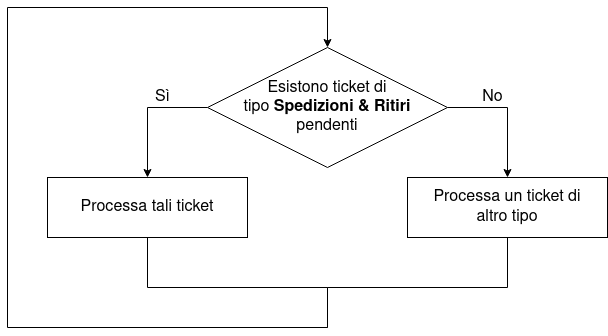
\includegraphics[width=0.75\linewidth]{presentazione-1}
\scaption{Schema del comportamento del servente dedicato ai ticket di tipo \textbf{Spedizioni \& Ritiri}}
\label{fig:presentazione-1}
\end{figure}
\section{Obiettivi dello studio}
L'obiettivo dello studio è quello di individuare ed analizzare gli indici prestazionali del sistema \textbf{Poste Italiane} e di proporre una miglioria nel sistema di processamento delle richieste, al fine di ridurre il tempo medio d'attesa sperimentato dai clienti in coda.

\end{document}